\documentclass[11pt,a4paper]{article}
\usepackage{fontspec}
\setmainfont{TeX Gyre Pagella}
\newfontfamily\headfont{Inter}[UprightFont=*-ExtraBold,BoldFont=*-ExtraBold,Extension=.otf,Path=/usr/share/fonts/opentype/inter/]
\usepackage[a4paper,margin=2.3cm]{geometry}
\usepackage{graphicx,booktabs,float,caption,array,xcolor}
\usepackage[hidelinks]{hyperref}
\usepackage{titlesec}
\usepackage{setspace}
\setstretch{1.05}
\renewcommand{\topfraction}{0.9}
\renewcommand{\bottomfraction}{0.8}
\renewcommand{\textfraction}{0.1}
\renewcommand{\floatpagefraction}{0.75}
\setlength{\parindent}{0pt}
\setlength{\parskip}{0.55em}
\titleformat{\section}{\headfont\Large}{\thesection}{0.8em}{}
\titleformat{\subsection}{\headfont\large}{\thesubsection}{0.8em}{}
\captionsetup{font=small,labelfont=bf}
\urlstyle{same}
\hypersetup{pdftitle={Where the Wind Blows},pdfauthor={Tristan Hotham}}

\begin{document}
\begin{center}
{\Large\bfseries Where the Wind Blows\\[2pt] The World's Winds Month by Month, Its Windiest Places, and Whether Wind Farms Stand in Them\par}
\vspace{1.2em}
{\large Tristan Hotham\par}
\vspace{0.3em}
{\small Independent researcher\\
ORCID: 0000-0003-4931-9349\\
DOI: \href{https://doi.org/10.5281/zenodo.23844511}{https://doi.org/10.5281/zenodo.23844511}\par}
\vspace{0.8em}
2026
\end{center}

\begin{quote}
\small
\begin{center}\textbf{Abstract}\end{center}
I map mean wind speed over the world's land month by month from WorldClim 2.1 (10 m above the ground, 1970 to 2000, 5 arc minutes) and set it beside the near-surface circulation of the NCEP/NCAR Reanalysis 1 (long-term means for 1991 to 2020, 2.5 degrees). Over the oceans the trade winds average 6.7 m/s in the north and 7.0 m/s in the south and are the steadiest winds on Earth; the Roaring Forties (40 to 50 degrees south) average 10.2 m/s against 8.8 m/s at the same northern latitudes; and the monsoon reverses the wind over 12\% of the area between 60 degrees north and south. Over land outside Antarctica the mean wind is 2.9 m/s; the windiest places are ice caps and ocean islands, led by Vatnajökull in Iceland (15.8 m/s). On northern land the windiest month is April, not midwinter. Setting the 5,344 wind farms of the WRI Global Power Plant Database (a 2021 snapshot) against the wind at their sites, 82\% of onshore capacity stands on ground windier than its country's median, and in 17 of 21 countries with substantial listed capacity the farms are windier than the national land average. The UK averages 4.9 m/s over land, 1.7 times the world's land average.

\textbf{Keywords:} wind; wind speed; atmospheric circulation; trade winds; westerlies; monsoon; seasonality; wind farms; WorldClim; NCEP/NCAR reanalysis; data visualisation
\end{quote}

\section{Introduction}

The winds of the world fall into belts that sailors named long before anyone could explain them: easterly trade winds either side of the equator, westerlies in the middle latitudes, and in the far south the Roaring Forties, where the westerlies circle the globe with almost no land in the way. In southern Asia and a few other regions the prevailing wind reverses between winter and summer, the monsoon. Over land the picture is broken up by mountains, coasts and the roughness of forests and towns, which slow the wind near the ground.

This note maps these patterns from two open climatologies and asks three questions of them. Where are the windiest places on land? How strongly does the wind change with the seasons, and when is it windiest? And do the world's wind farms, as listed in the WRI Global Power Plant Database, stand in the windier parts of their countries? The results are published with an interactive month by month map at \url{https://maps.tristanhotham.com/wind-map/}.

\section{Data}

\subsection{WorldClim 2.1 wind speed}
WorldClim 2.1 (Fick and Hijmans 2017) provides monthly mean wind speed at 10 m above the ground for 1970 to 2000 over the world's land, interpolated from weather station records with covariates. I use the 5 arc minute version (about 9 km at the equator), 3,160,018 land cells after removing 10,196 cells that lie more than one cell from any Natural Earth land (most of them over the Caspian Sea). WorldClim data are free for research and other non-commercial use with citation, and may not be redistributed. I therefore publish only derived pictures and summaries: the interactive map shows the 5 arc minute grids as images in colour classes (0.5 m/s wide up to 8 m/s), and reads out values from a 0.5 degree summary rounded to 0.5 m/s; the tables give area means and values at named points. The grids themselves are not redistributed.

\subsection{NCEP/NCAR Reanalysis 1}
The NCEP/NCAR Reanalysis 1 (Kalnay et al. 1996) assimilates observations into a fixed global weather model. NOAA's Physical Sciences Laboratory publishes long-term monthly means at the model's lowest level (sigma 0.995, roughly the lowest 40 m of the atmosphere) on a 2.5 degree grid. I use the means for 1991 to 2020 of the zonal and meridional wind and of the wind speed computed from daily vector winds. These data are in the public domain.

\subsection{Wind farms}
The Global Power Plant Database v1.3 (Global Energy Observatory et al. 2021) lists power plants with their primary fuel, capacity, position and, for some, commissioning year. It is a snapshot of 2021, published under CC BY 4.0. It contains 5,344 plants with primary fuel ``Wind'', 263 GW in 58 countries; 42\% have a commissioning year, from 1,975 to 2,020. Coverage is uneven: the United States, China and the United Kingdom hold 68\% of the listed capacity, while Germany (25 plants) and India appear with a small fraction of their actual fleets.

\subsection{Boundaries and places}
Countries, first-level divisions and populated places are from Natural Earth (1:10m and 1:50m); UK counties (England's ceremonial counties, Welsh preserved counties, Scottish council areas and Northern Ireland) from Office for National Statistics boundaries.

\section{Methods}

\textbf{Land averages.} The annual mean of each WorldClim cell is the mean of its twelve monthly values. Averages over areas weight each cell by the cosine of its latitude. ``Land'' excludes Antarctica (south of 60 degrees) unless stated. For countries, overseas territories that hold no listed farms are excluded (for example, the United States is the conterminous 48 states, France is metropolitan France).

\textbf{Seasonality.} For each land cell with an annual mean of at least 1.5 m/s, seasonality is the ratio of the windiest to the calmest monthly mean. 3,634 cells in which one month is below 0.35 or above 2.5 times the mean of its two neighbouring months were treated as station artefacts and excluded from this measure.

\textbf{Windiest places.} Land cells outside Antarctica were ranked by annual mean; a cell was kept if it lay at least 500 km from every cell already kept, giving distinct local peaks. Most seasonal places were found the same way with a 700 km spacing.

\textbf{Circulation.} From the NCEP fields I take ocean cells (less than 10\% land, judged from the WorldClim mask) and average by latitude band. Steadiness is the length of the annual mean wind vector divided by the annual mean wind speed: 1 if the wind always blew from one direction. Monsoon reversal is defined for 2.5 degree cells where both the January and the July mean vectors are at least 2 m/s and point at least 135 degrees apart.

\textbf{Wind farms.} A farm is on land if its point falls in a WorldClim land cell, on the coast if not but a neighbouring cell is land (its wind is then the mean of those cells), and at sea otherwise. For each onshore farm I compute its percentile: the share of its country's land area with a lower annual mean wind than the farm's cell. Country and global figures weight farms by capacity. Country comparisons are restricted to the 21 countries with at least 400 MW in 8 or more listed onshore farms.

\section{Results}

\subsection{The wind belts}
Figure \ref{fig:world} shows the annual mean wind with the mean near-surface flow, and Figure \ref{fig:months} four months of it. Over the oceans between 7.5 and 22.5 degrees, the trade winds blow from the north-east in the northern hemisphere (mean zonal wind -4.0 m/s, meridional -1.5) and from the south-east in the southern (-4.9 and 2.4). Their steadiness is 0.77, against 0.65 in the southern westerlies (40 to 55 degrees south) and 0.38 in the northern westerlies (Figure \ref{fig:belts}).

\begin{figure}[tbp]\centering
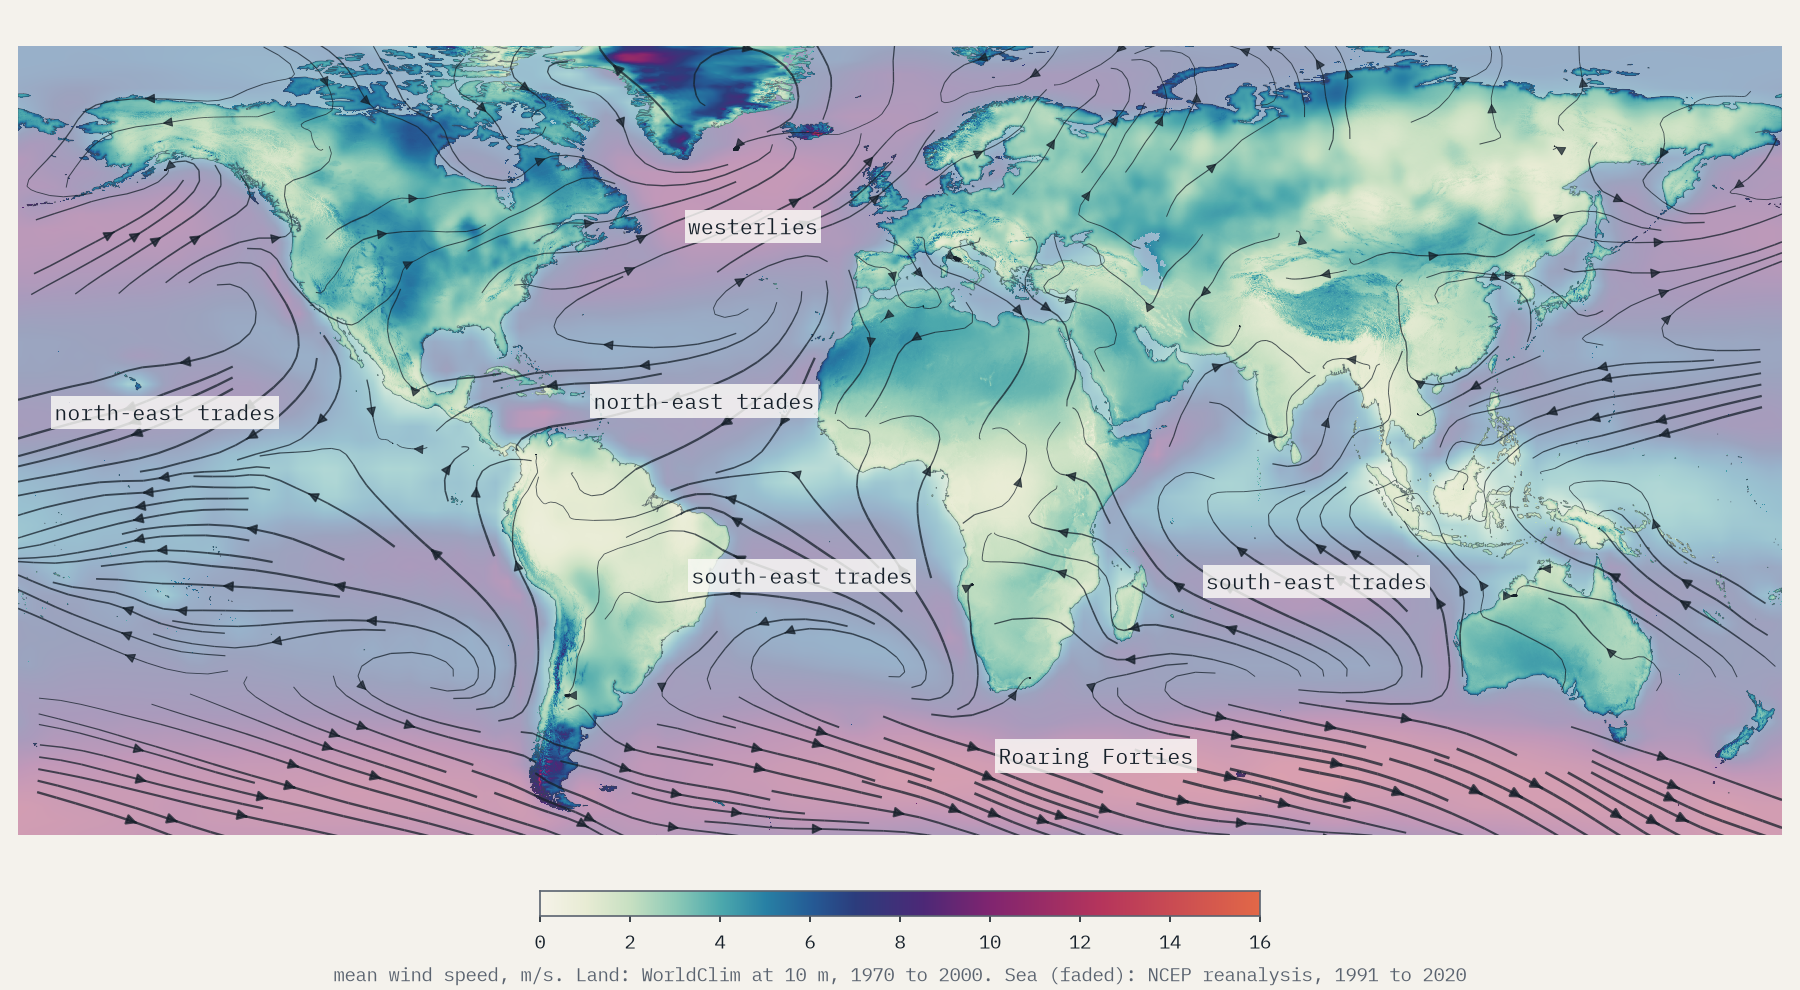
\includegraphics[width=\textwidth]{fig_world_map.png}
\caption{Annual mean wind speed. Land: WorldClim 2.1 at 10 m, 1970 to 2000. Sea (faded): NCEP/NCAR Reanalysis 1 near-surface wind speed, 1991 to 2020. Lines: streamlines of the annual mean near-surface wind vector from the reanalysis.}\label{fig:world}
\end{figure}

\begin{figure}[tbp]\centering
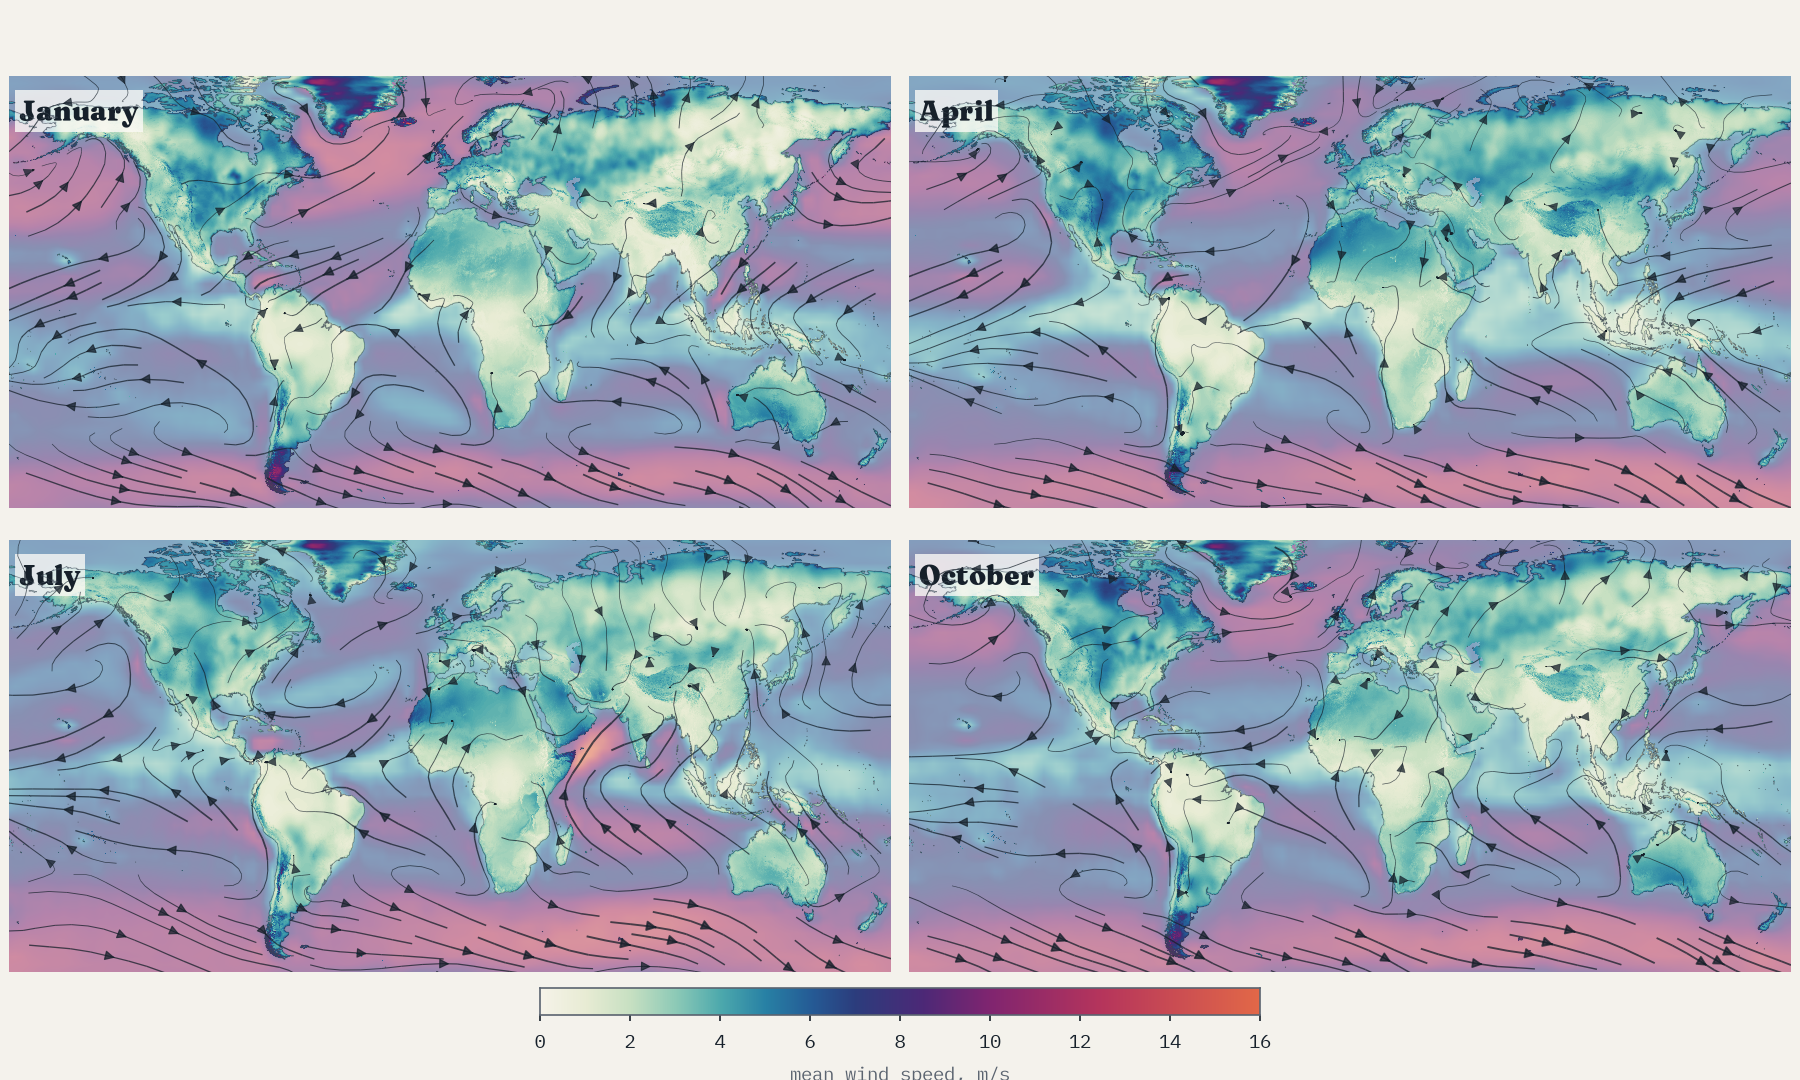
\includegraphics[width=\textwidth]{fig_months.png}
\caption{Mean wind speed and near-surface flow in January, April, July and October; sources as in Figure \ref{fig:world}.}\label{fig:months}
\end{figure}

The southern westerlies are the strongest belt: mean zonal wind 6.7 m/s against 3.1 m/s in the north. Over the ocean between 40 and 50 degrees south the mean speed is 10.2 m/s, against 8.8 m/s between 40 and 50 degrees north, a ratio of 1.15. The fastest latitude band is at 52.5 degrees south (11.4 m/s), and the windiest ocean cell lies in the southern Indian Ocean at 50.0 degrees south, 87.5 degrees east (12.6 m/s). The southern belt holds its strength through the year: in January the northern band is windier (10.3 against 9.5 m/s), but in July the northern band falls to 6.9 m/s while the southern rises to 10.9. Between 60 degrees north and south, the ocean wind averages 7.6 m/s; over solid land the same reanalysis gives 3.8 m/s.

\begin{figure}[tbp]\centering
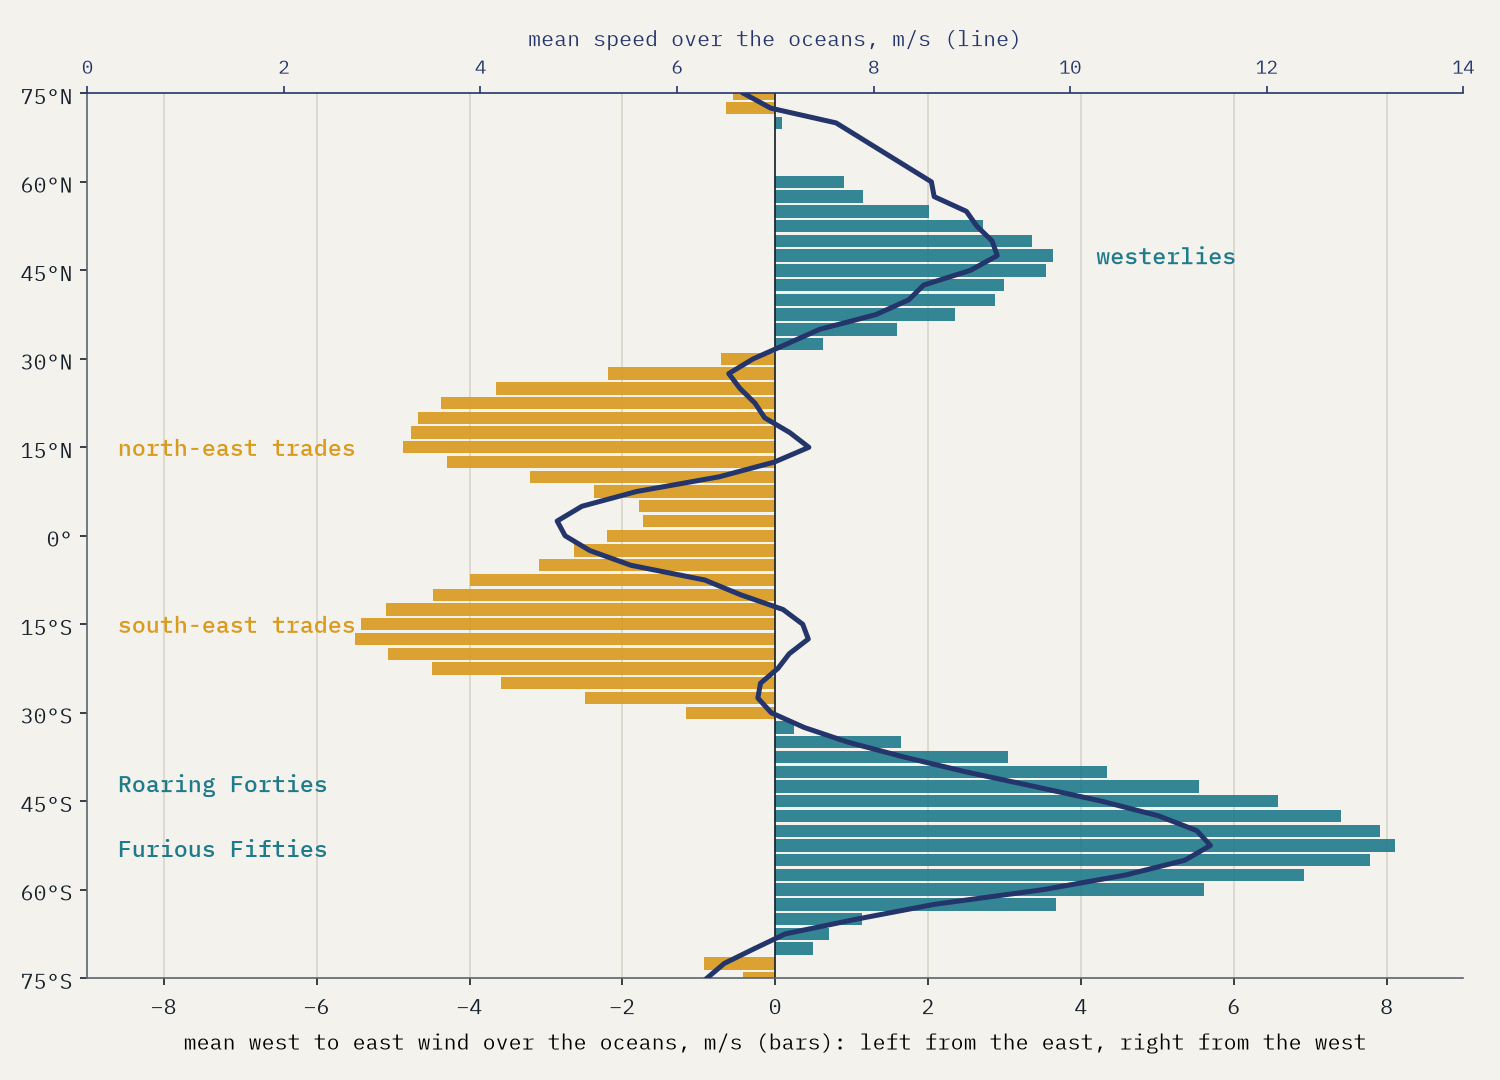
\includegraphics[width=0.86\textwidth]{fig_belts.png}
\caption{Mean zonal (west to east) wind over the oceans by latitude, NCEP/NCAR Reanalysis 1, 1991 to 2020 (bars; negative values are easterly), and mean wind speed (line).}\label{fig:belts}
\end{figure}

\subsection{The monsoon}
In the Arabian Sea (7.5 to 17.5 degrees north, 55 to 70 degrees east) the January mean wind is from the north-east at 6.3 m/s and the July mean wind from the south-west at 11.7 m/s (Figure \ref{fig:monsoon}). Off Somalia the July wind averages 13.6 m/s, the low-level Somali jet. The Bay of Bengal reverses in the same way, from the north-east in January to the south-west in July. By the definition above, 12\% of the area between 60 degrees north and south reverses its wind between January and July (749 cells).

\begin{figure}[tbp]\centering
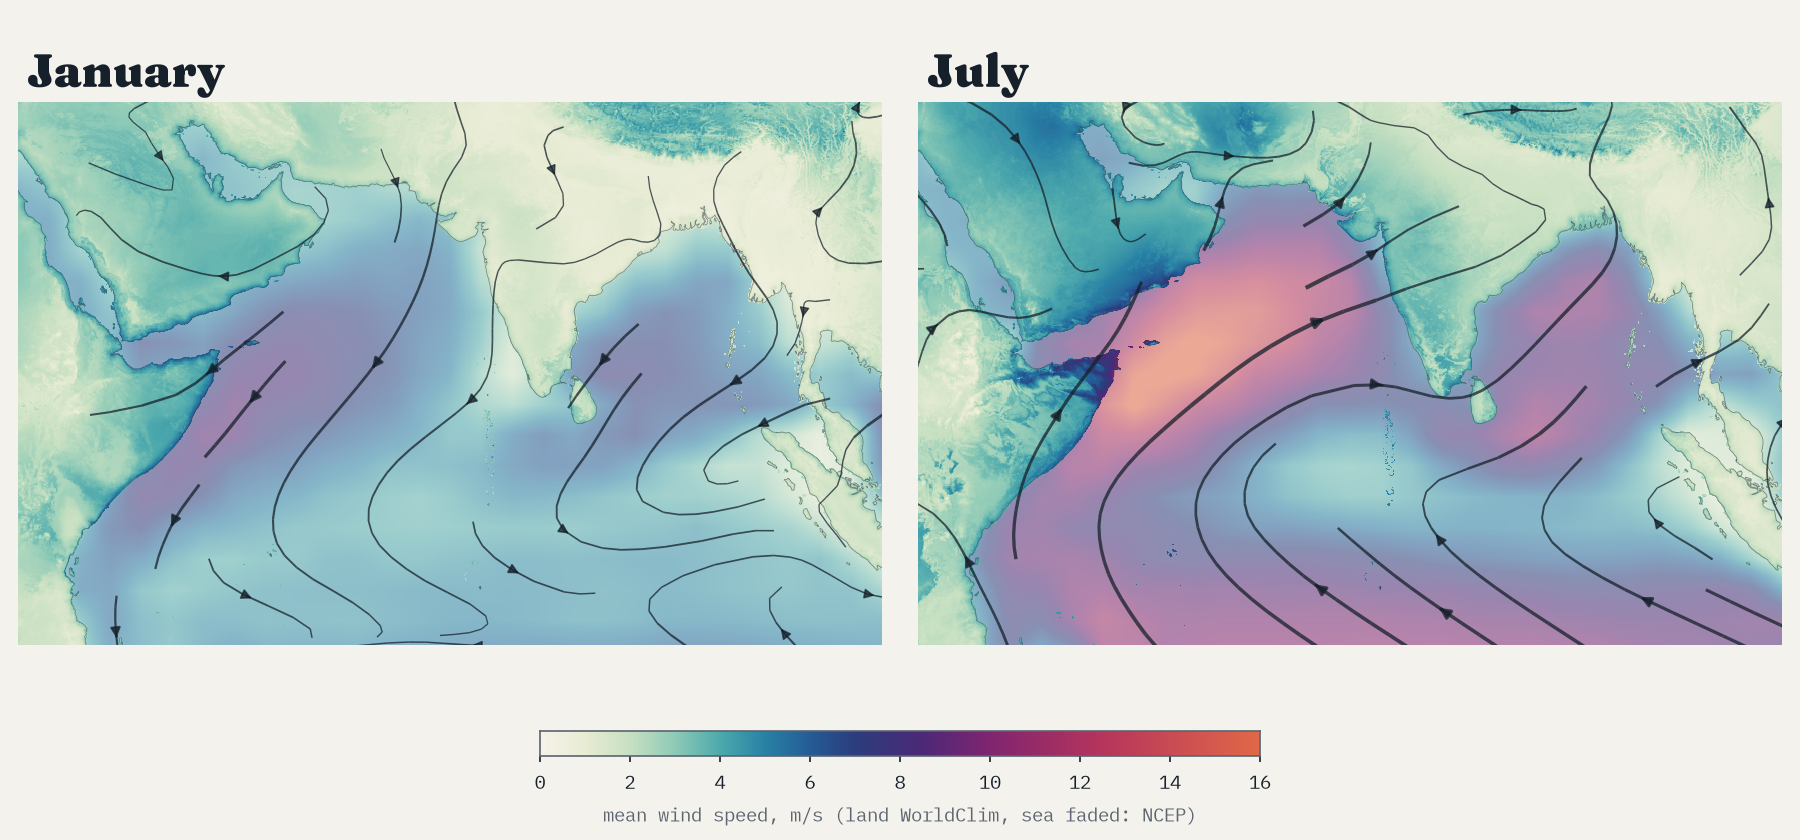
\includegraphics[width=\textwidth]{fig_monsoon.png}
\caption{The Indian Ocean in January and July: mean wind speed (land WorldClim; sea NCEP, faded) and mean near-surface flow.}\label{fig:monsoon}
\end{figure}

\subsection{Wind over land and the windiest places}
The mean wind over land outside Antarctica is 2.85 m/s (median 2.92); including Antarctica it is 3.16. Only 4.6\% of land outside Antarctica averages 5 m/s or more and 1.6\% 6 m/s or more, while 25\% averages under 2 m/s. Table \ref{tab:places} and Figure \ref{fig:windiest} list the 20 windiest distinct places. The first is the Vatnajökull ice cap in Iceland (15.8 m/s), followed by Jan Mayen, the East Greenland ice sheet and the Southern Patagonian Ice Field; the rest are ice fields, high Andes and sub-Antarctic islands, with St Kilda the only point in the British Isles. Antarctica reaches 20.0 m/s. These are also the places with the sparsest station networks, where the interpolated values are least certain. Among countries and territories of at least 50,000 km\textsuperscript{2}, Iceland is windiest (6.7 m/s) and the Republic of the Congo calmest (1.1 m/s).

\begin{table}[tbp]\centering\small\caption{The 20 windiest distinct places on land outside Antarctica: annual mean wind at 10 m (WorldClim 2.1, 1970 to 2000), each at least 500 km from any windier one, with the windiest month.}\label{tab:places}\begin{tabular}{rllrrl}\toprule & Place & Country or territory & Lat, lon & m/s & Peak\\\midrule
1 & Vatnajökull ice cap & Iceland & 64.62, -17.54 & 15.8 & Jan \\
2 & Jan Mayen & Norway & 71.04, -8.21 & 13.6 & Jan \\
3 & East Greenland ice sheet & Greenland & 68.88, -29.88 & 13.5 & Feb \\
4 & Southern Patagonian Ice Field & Chile & -50.62, -73.29 & 13.1 & Jun \\
5 & North-west Greenland & Greenland & 77.79, -54.96 & 11.0 & Nov \\
6 & Cordillera Darwin, Tierra del Fuego & Chile & -54.62, -69.71 & 11.0 & Nov \\
7 & Heard Island & Australia & -53.12, 73.71 & 10.4 & Aug \\
8 & Macquarie Island & Australia & -54.71, 158.88 & 10.3 & May \\
9 & High Andes of Mendoza & Argentina & -33.38, -69.79 & 10.2 & Jun \\
10 & Bouvet Island & Norway & -54.38, 3.29 & 9.6 & Mar \\
11 & South Sandwich Islands & UK overseas territory & -59.46, -27.12 & 9.5 & Sep \\
12 & Campbell Island & New Zealand & -52.46, 169.12 & 9.3 & May \\
13 & South Greenland, near Narsarsuaq & Greenland & 61.79, -44.46 & 9.3 & Feb \\
14 & Norway's west coast, Sogn og Fjordane & Norway & 61.88, 4.79 & 9.2 & Jan \\
15 & Kerguelen Islands & France & -49.29, 69.62 & 9.2 & Aug \\
16 & Rat Islands, Aleutians & United States & 51.88, 179.71 & 9.0 & Jan \\
17 & Northern Patagonian Ice Field, Aysén & Chile & -46.12, -71.88 & 9.0 & Jan \\
18 & St Kilda & United Kingdom & 57.79, -8.62 & 8.8 & Jan \\
19 & Faroe Islands & Denmark & 62.29, -7.21 & 8.8 & Jan \\
20 & Fiordland & New Zealand & -45.54, 167.12 & 8.8 & May \\
\bottomrule\end{tabular}\end{table}

\begin{figure}[tbp]\centering
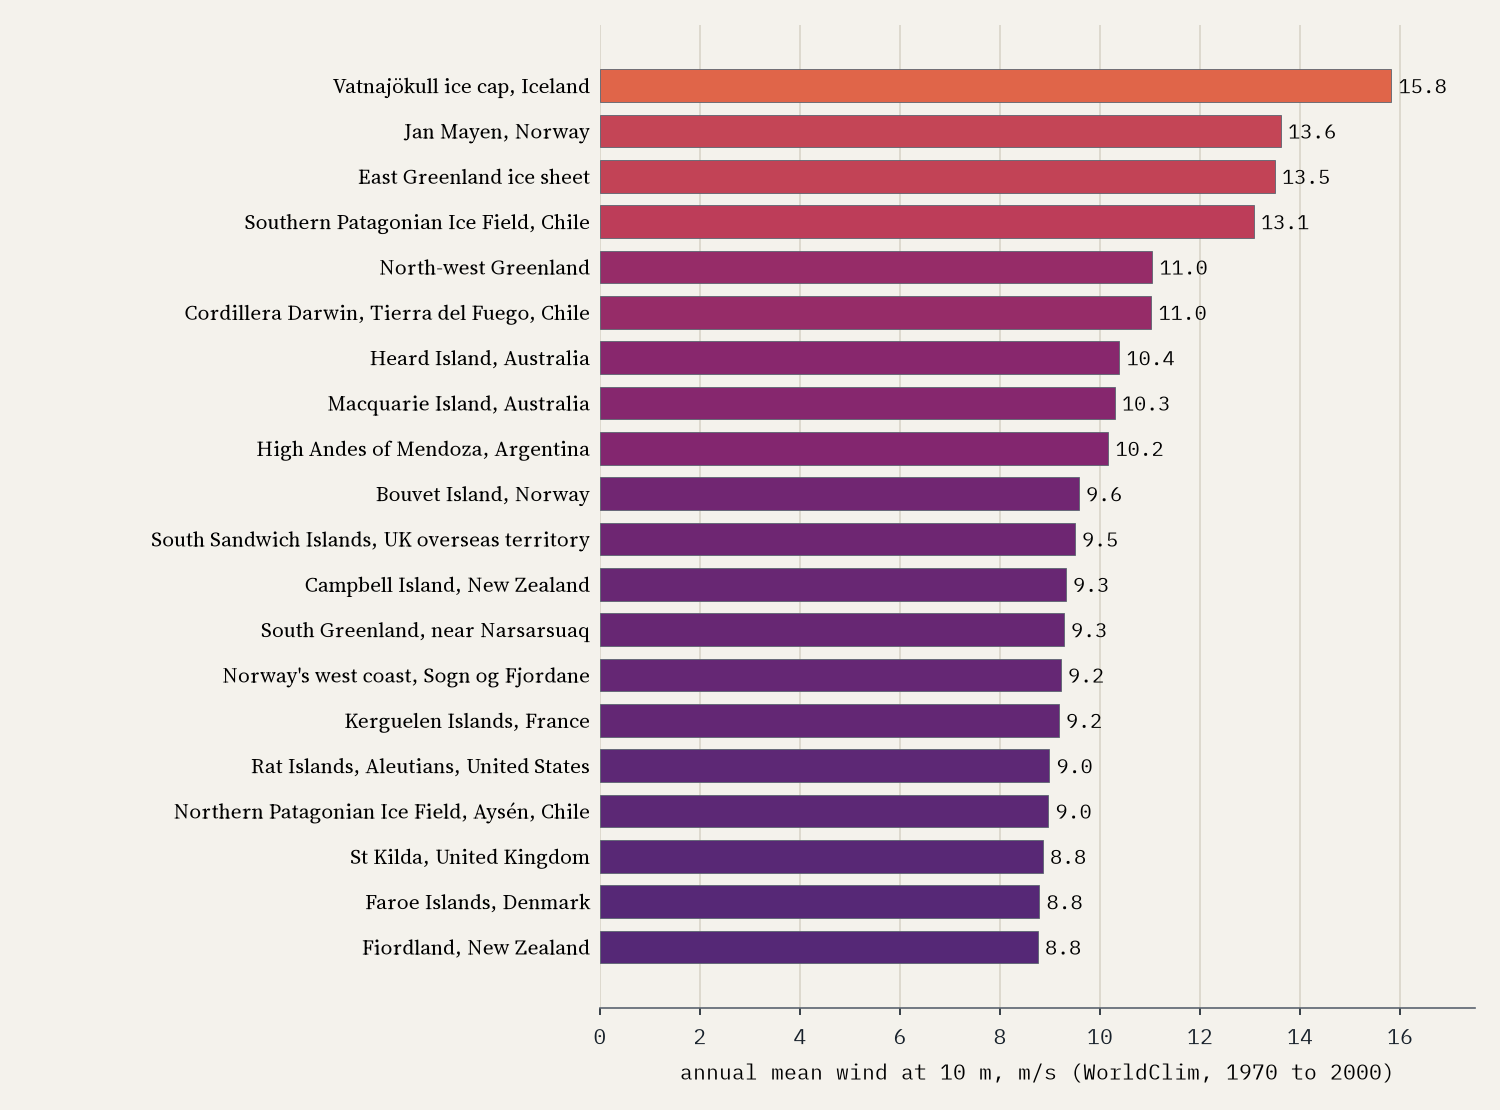
\includegraphics[width=0.86\textwidth]{fig_windiest.png}
\caption{The 20 windiest distinct places on land outside Antarctica, by annual mean wind at 10 m (WorldClim, 1970 to 2000).}\label{fig:windiest}
\end{figure}

Of the 505 Natural Earth cities with a million people or more, the windiest are Marseille (5.8 m/s), The Hague (5.6), Melbourne, Auckland and Adelaide; the calmest Bogotá (0.9), Cali, Srinagar, Medellín and Mandalay.

\subsection{Seasonality}
Averaged over northern land, the windiest month is April and the calmest August; over southern land outside Antarctica, October and May (Figure \ref{fig:seasons}). Spring is the windy season: 57\% of northern land beyond the tropics has its windiest month in March, April or May, and 28\% in April alone, against 30\% in December to March. The median ratio of the windiest to the calmest month is 1.48; 8\% of the land considered has a ratio of 2 or more and 16\% a ratio under 1.3. The highest ratios are in two kinds of place: the interior of north-eastern Siberia, Mongolia and the Yukon, where winter air is calm under the Siberian and North American highs (the Kolyma uplands of Yakutia reach 10.3), and the monsoon coasts and islands of the Indian Ocean (Kutch, Odisha, the Maldives and the Chagos Archipelago). Sistan, on the border of Afghanistan and Iran, peaks in July with its ``wind of 120 days''.

\begin{figure}[tbp]\centering
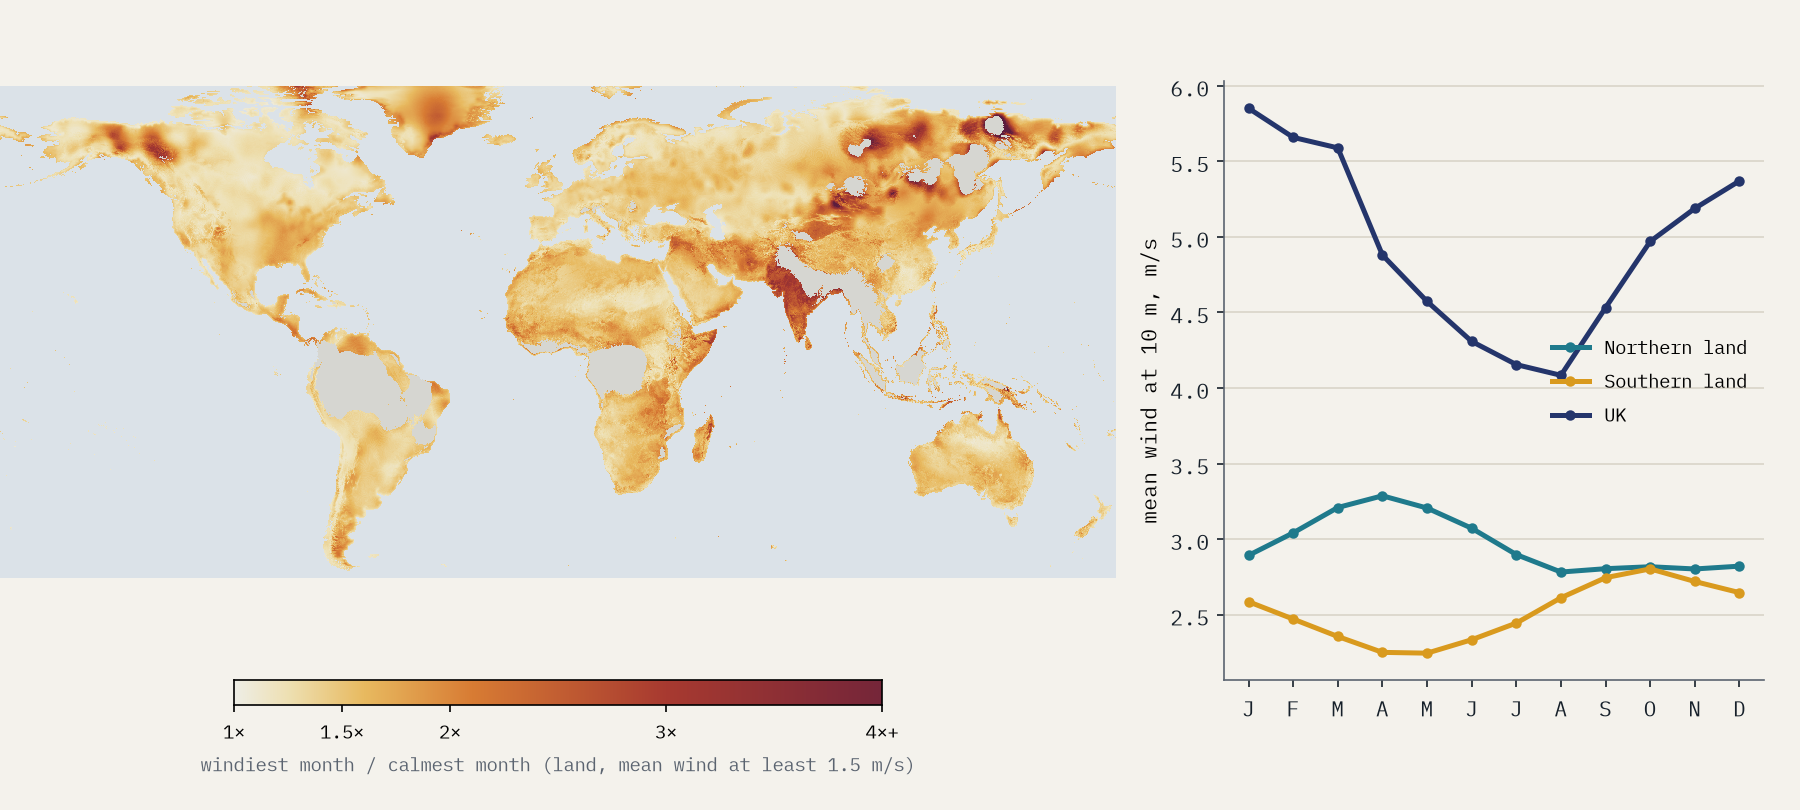
\includegraphics[width=\textwidth]{fig_seasons.png}
\caption{Left: ratio of the windiest to the calmest monthly mean wind (land with an annual mean of at least 1.5 m/s; grey: below). Right: area-weighted monthly mean wind over northern land, southern land (outside Antarctica) and the UK.}\label{fig:seasons}
\end{figure}

\subsection{Wind farms}
Of the 263 GW listed, 246.7 GW is on land cells, 2.8 GW on the coast and 13.5 GW at sea. Capacity-weighted, the average onshore farm stands at the 72\% point of its country's distribution of land wind: 82\% of onshore capacity is above the national median and 53\% in the windiest quarter of the land. The capacity-weighted mean wind at onshore farms is 3.93 m/s, 1.38 times the world land mean, though this comparison mixes countries. Among farms with a commissioning year, those from 2010 onwards stand at the 77\% point and earlier ones at the 71\% point.

Table \ref{tab:farms} and Figure \ref{fig:farms} give the 21 countries with substantial listed onshore capacity. In 17 the farms are windier on average than the land. The largest differences are in countries where good wind resources are concentrated: Mexico, whose listed farms are almost all in the Isthmus of Tehuantepec in Oaxaca (98\%), Brazil, mostly along the north-east coast (2.44 m/s against 1.50), and Australia and Norway. The United States (4.35 against 3.62) and China (3.36 against 2.74) follow, with farms concentrated on the Great Plains and in Inner Mongolia and Gansu. Chile is the clearest exception (31\%): its farms are in the north and centre, near demand and the grid, while its windiest land is in Patagonia. In the UK the farms are only modestly windier than the land (5.22 against 4.93 m/s), as its windiest ground is islands and uplands.

\begin{table}[tbp]\centering\small\caption{Countries with at least 400 MW in 8 or more listed onshore wind farms (WRI Global Power Plant Database, 2021): onshore farms and capacity, capacity at sea, mean wind at 10 m over the land and capacity-weighted at the onshore farms (m/s), the farms' mean percentile in the country's land wind, and the share of onshore capacity in the windiest quarter of the land (\%).}\label{tab:farms}\begin{tabular}{lrrrrrrr}\toprule Country & Farms & MW land & MW sea & Land & Farms & Pctile & Top quarter\\\midrule
United States & 1139 & 104,477 & 0 & 3.62 & 4.35 & 76 & 60\\
China & 830 & 50,594 & 0 & 2.74 & 3.36 & 73 & 51\\
United Kingdom & 742 & 13,946 & 7,442 & 4.93 & 5.22 & 61 & 35\\
Canada & 241 & 12,134 & 0 & 3.75 & 3.99 & 59 & 14\\
Spain & 342 & 11,337 & 0 & 3.13 & 3.27 & 58 & 37\\
Brazil & 412 & 10,295 & 0 & 1.50 & 2.44 & 88 & 86\\
France & 721 & 9,063 & 0 & 3.65 & 4.08 & 67 & 46\\
Australia & 65 & 5,739 & 0 & 3.20 & 4.27 & 85 & 78\\
Germany & 13 & 1,626 & 3,433 & 3.43 & 3.94 & 69 & 53\\
Portugal & 223 & 4,940 & 0 & 3.02 & 3.16 & 61 & 37\\
India & 108 & 3,647 & 0 & 1.74 & 2.26 & 81 & 69\\
Poland & 59 & 2,174 & 0 & 3.26 & 3.45 & 63 & 37\\
South Africa & 24 & 2,031 & 0 & 2.76 & 3.36 & 79 & 64\\
Netherlands & 35 & 762 & 1,174 & 4.36 & 5.03 & 68 & 65\\
Mexico & 20 & 1,587 & 0 & 2.54 & 3.82 & 98 & 100\\
Uruguay & 39 & 1,382 & 0 & 3.31 & 3.42 & 57 & 32\\
Ireland & 38 & 1,287 & 0 & 4.55 & 4.39 & 48 & 12\\
Morocco & 11 & 1,210 & 0 & 4.06 & 3.90 & 47 & 4\\
Chile & 18 & 897 & 0 & 4.74 & 3.45 & 31 & 0\\
Sweden & 8 & 577 & 0 & 3.08 & 2.93 & 47 & 15\\
Norway & 10 & 623 & 0 & 3.86 & 5.21 & 84 & 87\\
\bottomrule\end{tabular}\end{table}

\begin{figure}[tbp]\centering
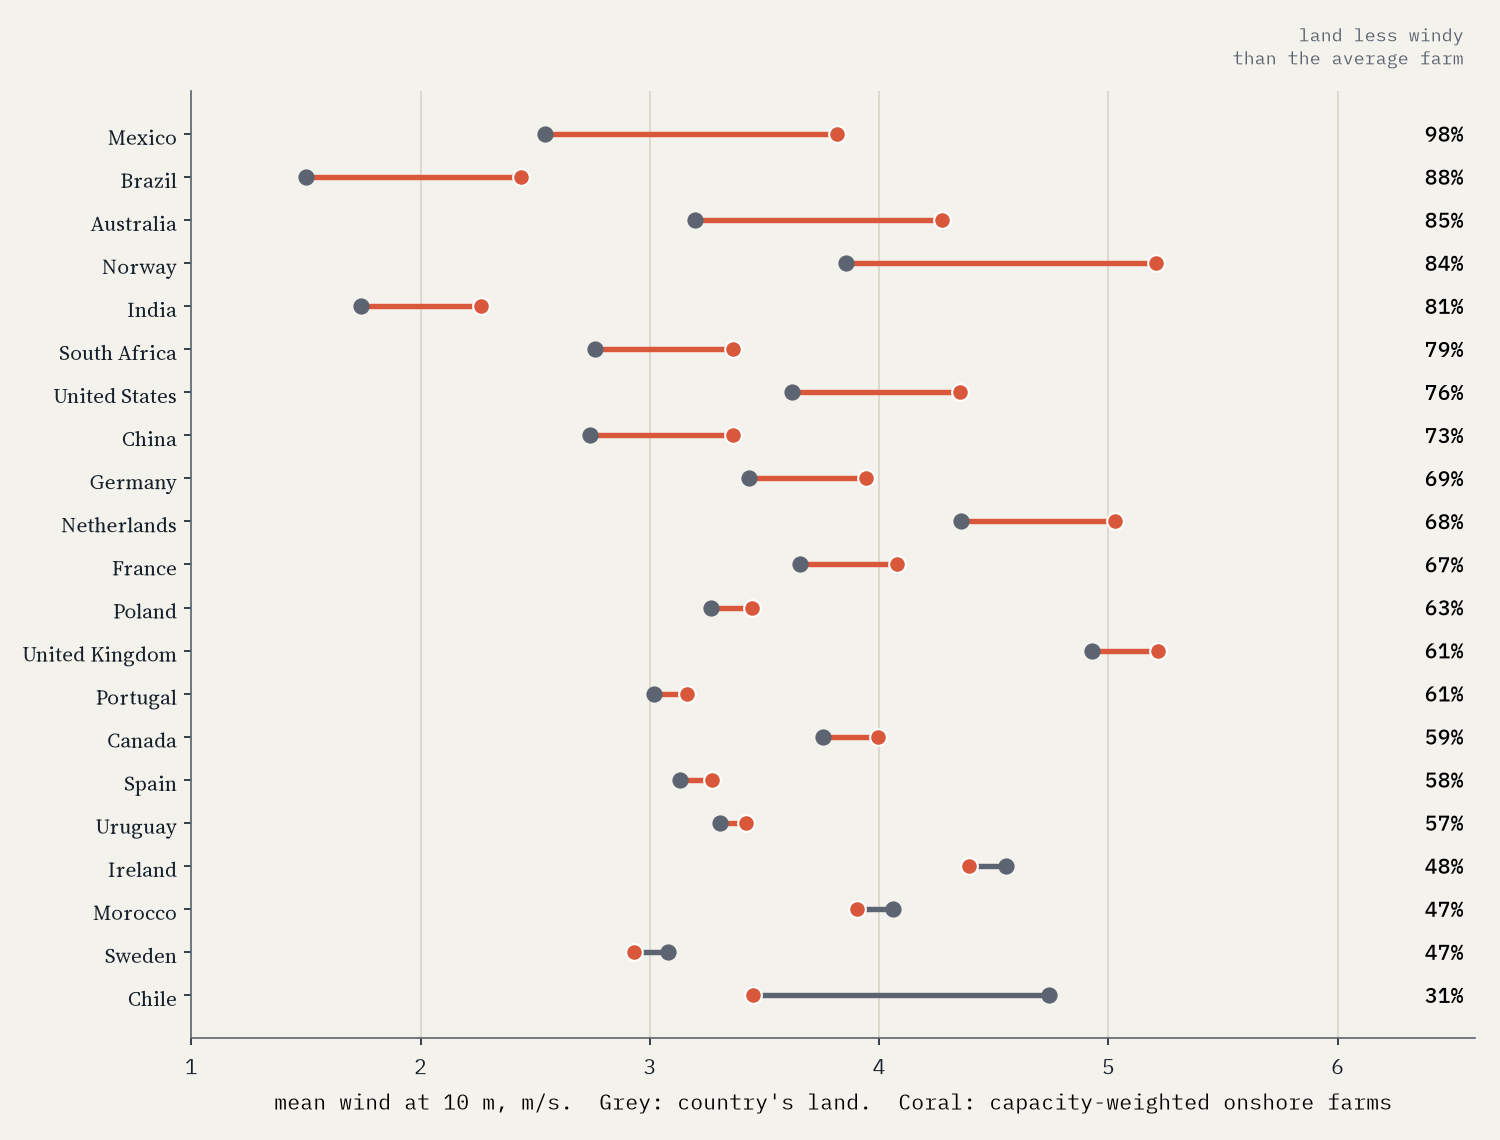
\includegraphics[width=0.9\textwidth]{fig_farms.png}
\caption{Mean wind at 10 m over each country's land (grey) and the capacity-weighted mean at its listed onshore wind farms (coral), with the share of the country's land less windy than the average farm.}\label{fig:farms}
\end{figure}

\subsection{The United Kingdom and Ireland}
The UK's land averages 4.93 m/s at 10 m (Scotland 5.63, England 4.59, Wales 4.61, Northern Ireland 4.61); Ireland averages 4.55. Among countries and territories of at least 50,000 km\textsuperscript{2}, only Iceland, Greenland and Western Sahara are windier than the UK. 41\% of UK land averages 5 m/s or more. The windiest counties are Shetland (7.60), Na h-Eileanan Siar, Orkney, Argyll and Bute and North Ayrshire; in England, Cornwall (5.99), Cumbria and the East Riding of Yorkshire; the calmest are Herefordshire (3.34), Shropshire and Worcestershire. The windiest cell is St Kilda (8.9 m/s). The UK's wind peaks in January (5.85 m/s) and is lowest in August (4.08), a ratio of 1.43. The database lists 780 UK wind farms with 23.2 GW, of which 7.4 GW (32\%) is at sea; Scotland holds 61\% of the onshore capacity (Figure \ref{fig:uk}).

\begin{figure}[tbp]\centering
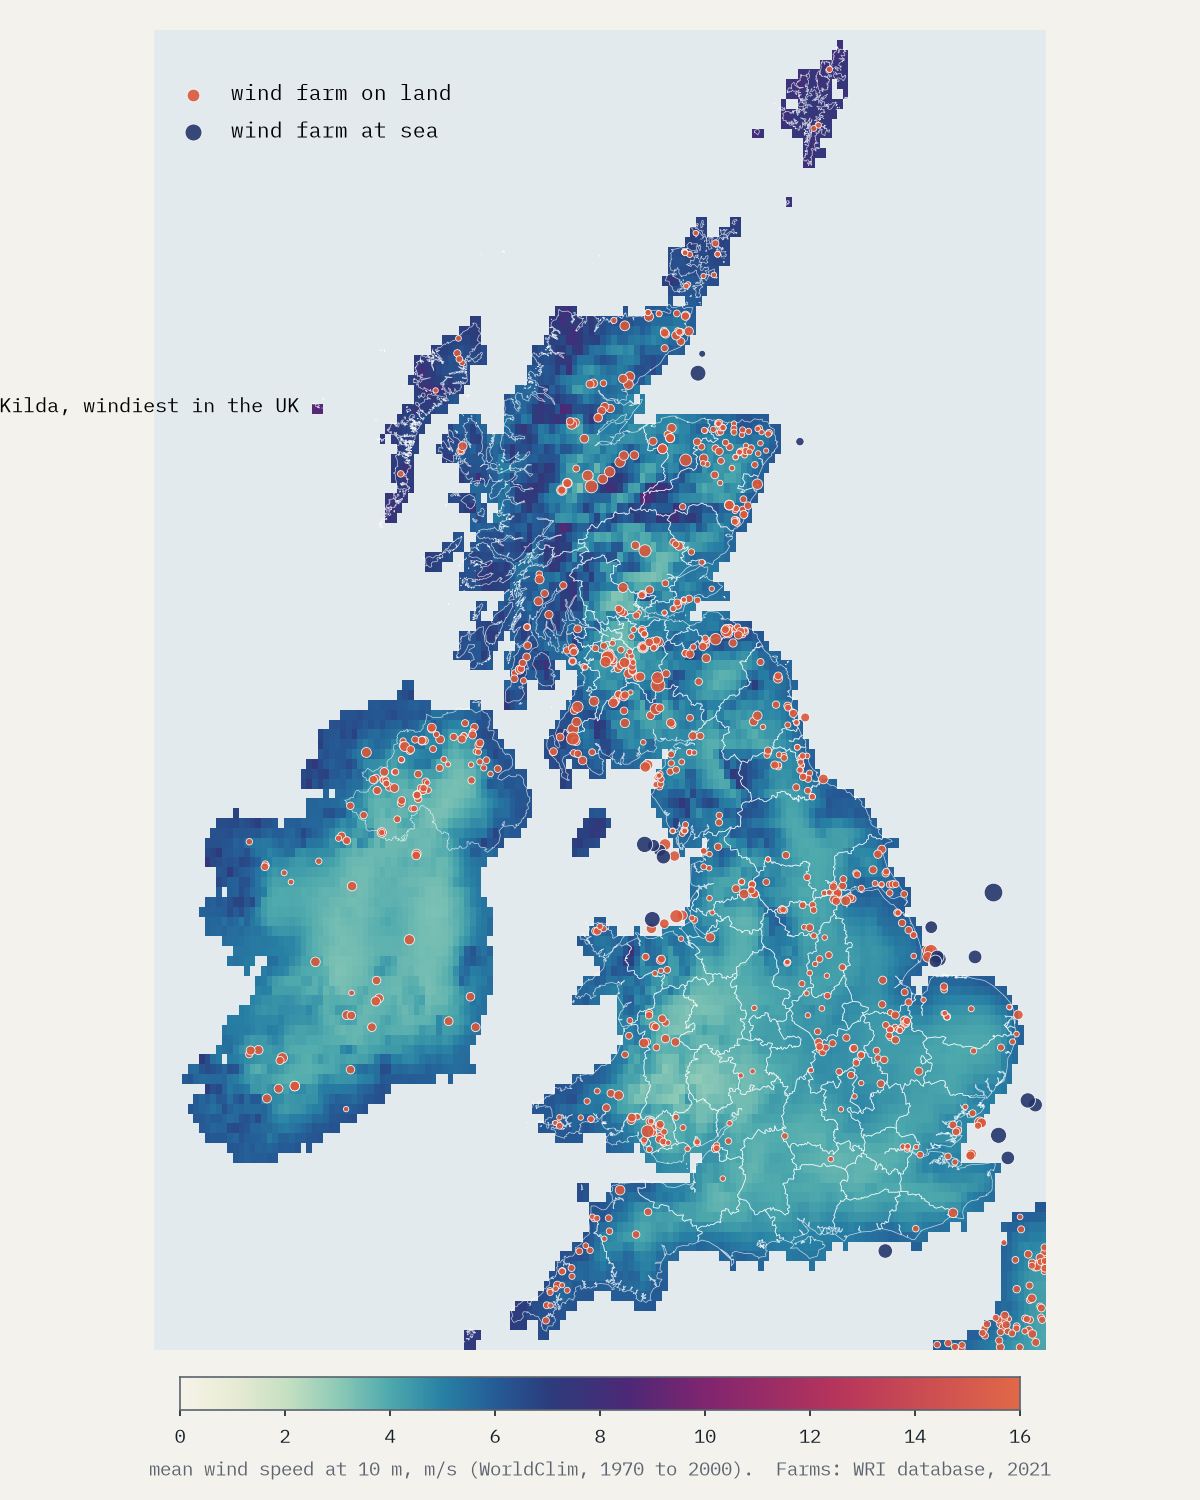
\includegraphics[width=0.72\textwidth]{fig_uk.png}
\caption{Annual mean wind at 10 m over the UK and Ireland (WorldClim, 1970 to 2000) with wind farms from the WRI Global Power Plant Database (2021): on land (coral) and at sea (navy), sized by capacity.}\label{fig:uk}
\end{figure}

\section{Discussion and limitations}
The two climatologies differ in height, resolution and period. Over 2,017 cells of solid land the reanalysis wind speed is a median 1.39 times the WorldClim value, while the two agree on where it is windy (correlation 0.79); I therefore use the reanalysis only for direction and the oceans, and draw it faded. WorldClim's 10 m wind is not the wind at a turbine hub, 80 to 150 m up, and a 9 km cell averages over the ridges and hilltops where farms are built, so the farm comparisons are conservative and say nothing about energy yield, which depends on the distribution of wind speeds rather than the mean. The interpolation is weakest where stations are few: ice caps, mountains, deserts and remote islands, which dominate the list of windiest places. The power plant database is a 2021 snapshot, incomplete for several large markets, and its points can be approximate. Siting reflects much more than wind: grid access, land, planning and demand, as Chile and the UK show.

\section{Conclusion}
Two open climatologies are enough to draw the classic belts of the world's winds and the seasonal reversal of the monsoon, and to show that, with few exceptions, the world's listed wind farms stand on the windier ground of their countries: 82\% of onshore capacity is above the national median.

\section*{Data and code availability}
Code, derived data and the interactive page: \url{https://github.com/Tristan-Hotham/wind-map} and \url{https://maps.tristanhotham.com/wind-map/}. Archived release with this paper: \url{https://doi.org/10.5281/zenodo.23844511}. Derived data and text are CC BY 4.0, except that summaries derived from WorldClim are for non-commercial use under the WorldClim terms; code is MIT.

\section*{AI statement}
I wrote the text, with drafting and editing assistance from Claude (Anthropic), which also helped prepare the analysis code. I reviewed and checked all text and results.

\section*{References}
\small
\begin{description}\setlength{\itemsep}{2pt}
\item Fick, S.E. and Hijmans, R.J. (2017) WorldClim 2: new 1 km spatial resolution climate surfaces for global land areas. International Journal of Climatology 37(12): 4302 to 4315. \url{https://doi.org/10.1002/joc.5086}
\item Global Energy Observatory, Google, KTH Royal Institute of Technology in Stockholm, Enipedia, World Resources Institute (2021) Global Power Plant Database v1.3.0. \url{https://datasets.wri.org/dataset/globalpowerplantdatabase} (CC BY 4.0).
\item Kalnay, E., Kanamitsu, M., Kistler, R. et al. (1996) The NCEP/NCAR 40-year reanalysis project. Bulletin of the American Meteorological Society 77(3): 437 to 471.
\item NOAA Physical Sciences Laboratory. NCEP/NCAR Reanalysis 1, long-term monthly means at sigma 0.995. \url{https://psl.noaa.gov/data/gridded/data.ncep.reanalysis.derived.html}
\item Natural Earth. Free vector and raster map data. \url{https://www.naturalearthdata.com}
\end{description}
\end{document}
